\chapter{Methods}
    \label{cha:methods}
    %

    %
    \section{Chromatin Specifications}
        \label{sec:ChromatinModel}

        %
        The chromatin model in this work can be reduced, so that a nucleosome is modelled as one single amino acid (e.g. $K27$) which can be either acetylated (referred to as active) or monomethylated (referred to as silenced). Di- and trimethylation will not be featured in this work.
        %

        %
        The nucleosome string is either modelled to be non-cyclic (as done in \ref{sec:ResNon-cooperative} and \ref{sec:ResNonCyc}) or cyclic (\ref{sec:ResBistableSwitching} to \ref{sec:ResBoundariesBistability}). In the cyclic case, the enzymes' pattern can include nucleosomes from the start as well as the end of the string simultaneously. In the non-cyclic case, the first and last nucleosome logically only have one neighbour.
        %

        %
        The non-cyclic models contain 60 nucleosomes whereas the cyclic ones only contain 40 nucleosomes in order to reduce computation time and storage space.
        %

        %
        The starting state for every simulation in this work is a completely unmodified nucleosome string. As long as there are random adders in the system (which is the case for every system featured in this work), the completely unmodified string logically is an unstable configuration which does not offer any sort of bias in the direction of acetylation or methylation respectively, hence the choice of an entirely unmodified starting state. The time it takes for the system to adjust in order to establish a fully modified string is negligible compared to the total time of one simulation run.
        %
    %
    %
    \section{Enzyme specifications}
    \label{sec:EnzymeTypes}
        %

        %
        All enzyme adder rules exclusively work on an unmodified nucleosome. Accordingly, for instance, a methylated nucleosome must be demodified first before an \ac/ adder enzyme can acetylate it. The opposite counts for an acetylated nucleosome. In summary, the modification pathway $ac \longleftrightarrow un \longleftrightarrow  me$ is imperative for all enzyme rules.
        %

        %
        The enzyme rule sets as well as their rates were defined symmetrically throughout the entirety of the simulations that were done for this work. Thus, for instance, every rule which defines the addition of an acetyl group to a nucleosome next to one that already has an acetyl group is defined in either direction on the string and has a methylation counterpart at equal association and dissociation rates.
        %

        %
        One of the strengths of Gillespie's algorithm is the possibility of emulating a system where molecule concentrations are very low, to the extent that they deplete over time. To that effect, the association rate (not the dissociation rate) set in the enzyme rule set is normally multiplied by the given concentration in the conventional SSA. Concentration depletion effects provided as a feature by \ed/ were not used in this work. Accordingly, all enzymes were assumed to be equally and infinitely available in the simulation. Supposing that there are more enzymes of one type in the system than could ever bind onto the string simultaneously, this seems to be an appropriate approximation. As a result, the concentration is supposed to be 1 for each enzyme rendering the assciation rates and dissociation rates directly comparable to each other.
        %

        %
        A short summary of all enzyme types featured in this work can be found in tab. \ref{img:enzymeTypeSummary}.
        %

        %
        \subsection{Enzyme types}

            %
            \subsubsection{Linear modifier enzymes}
                %

                %
                Linear modifier enzymes are used to extending sites which contain a specific modification (e.g. acetylation, see fig. \ref{img:linearEnzymes}) by either propagating said modification from nucleosome to neighbouring unmodified nucleosome (fig. \ref{img:linearEnzymes} \textbf{(a)}) or by deleting an opposing modification next to a nucleosome with the desired one (fig. \ref{img:linearEnzymes} \textbf{(b)}). They always have direct neighbour reach.
                %

                %
                \begin{figure}[htpb!]
                    \centering
                    \begin{minipage}[t][5cm]{\textwidth}
                        \begin{minipage}{0.15\textwidth}
                            \caption*{\small \textbf{(a)}}
                        \end{minipage}
                        \begin{minipage}{0.8\textwidth}
                            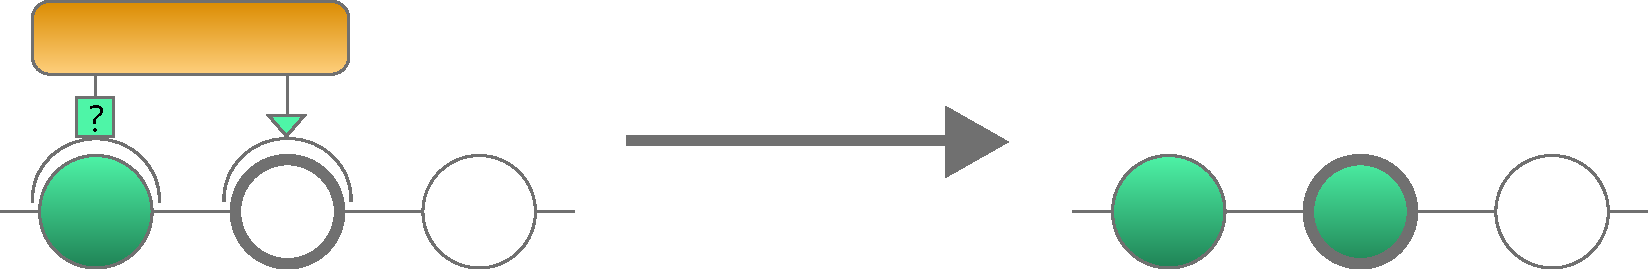
\includegraphics[width=\textwidth]{enzymes/linear_a.pdf}
                        \end{minipage}
                        \vfill
                        \begin{minipage}{0.15\textwidth}
                            \caption*{\small \textbf{(b)}}
                        \end{minipage}
                        \begin{minipage}{0.8\textwidth}
                            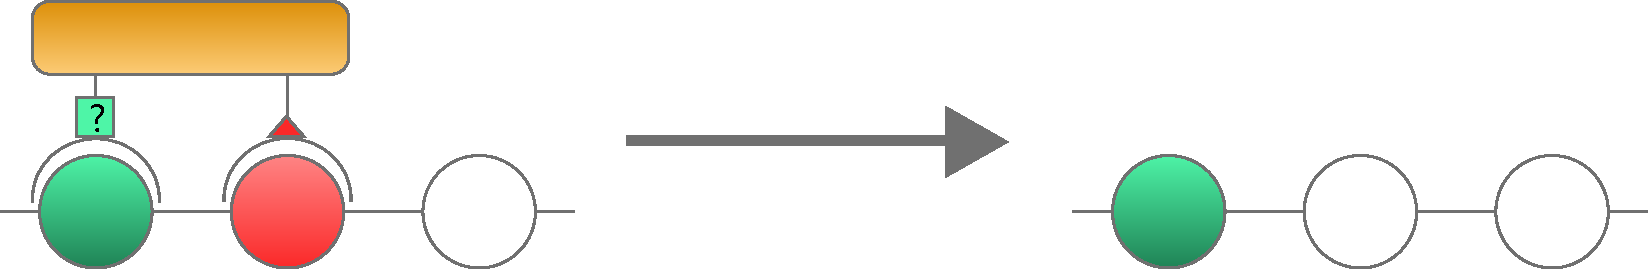
\includegraphics[width=\textwidth]{enzymes/linear_b.pdf}
                        \end{minipage}
                    \end{minipage}
                    \caption{Simplified model of linear modifier enzyme \textbf{(a)} acetylation addition and \textbf{(b)} methylation removal reactions. Acetylated nucleosomes are coloured in green, methylated nucleosomes are red and colourless ones are unmodified. The reactions shown are also defined in the rule set to occur in the opposite direction. Linear modifier enzymes in favour of methylation extension (or acetylation deletion) work analogically.}
                    \label{img:linearEnzymes}
                \end{figure}
                %
            %
            %
            \subsubsection{Cooperative modifier enzymes}
                \label{subsubsec:coopEnzymes}
                %

                %
                \begin{figure}[htpb!]
                    \centering
                    \begin{minipage}[t][3cm]{\textwidth}
                        \begin{minipage}{0.15\textwidth}
                            \caption*{\small \textbf{(a)}}
                        \end{minipage}
                        \begin{minipage}{0.8\textwidth}
                            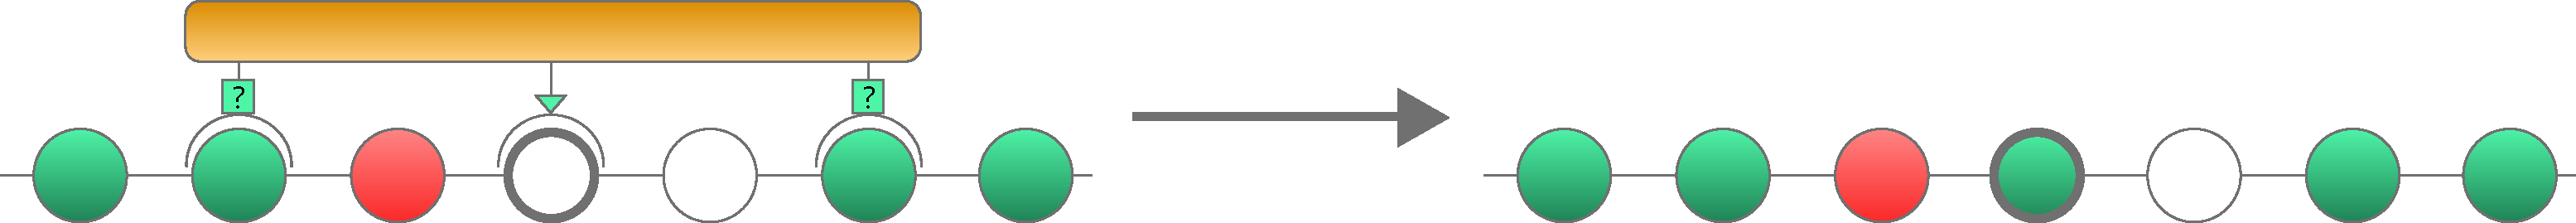
\includegraphics[width=\textwidth]{enzymes/coop_a.pdf}
                        \end{minipage}
                    \vfill
                        \begin{minipage}{0.15\textwidth}
                            \caption*{\small \textbf{(b)}}
                        \end{minipage}
                        \begin{minipage}{0.8\textwidth}
                            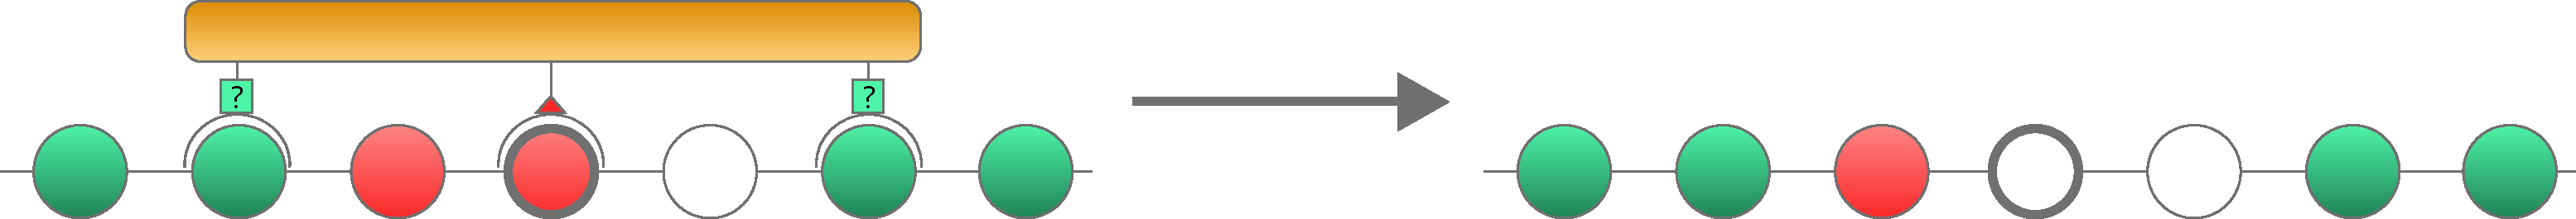
\includegraphics[width=\textwidth]{enzymes/coop_b.pdf}
                        \end{minipage}
                    \end{minipage}
                    \caption{Simplified model of cooperative modifier enzyme \textbf{(a)} acetylation addition and \textbf{(b)} methylation removal reactions. Acetylated nucleosomes are coloured in green, methylated nucleosomes are red and colourless ones are unmodified. The reactions shown are also defined in the rule set to occur in the opposite direction. Cooperative modifier enzyme methylation addition and acetylation removal work analogically.}
                    \label{img:coopEnzymes}
                \end{figure}
                %

                %
                Cooperative modifier enzymes generally read the state of two different nucleosomes on the string and write to or remove a modification from a third nucleosome. It is important to note that the two nucleosomes that are read do not need to have next-neighbour relation to the one the enzyme is modifying.  Thus, to some extent, these enzymes, unlike any other enzyme featured in this work, take the global modification trend on the string into account: if many nucleosomes are acetylated, then cooperative modifier enzymes in favour of acetylation (meaning cooperative acetylation adders and cooperative methylation removers) are more active which, in turn, reinforces the acetylation distribution on the string.
                %

                %
                The cooperative modifier enzymes in this work are implemented in a way that they are always reading two nucleosomes that are equally far away from the nucleosome the enzyme wants to modify (see fig. \ref{img:coopEnzymes}).
                %

                %
                The notion of 'space' of a cooperative enzyme defines the pattern reach of said enzyme. For instance, a cooperative adder with a reach of three will read the nucleosome it wants to write on and ignore the three next neighbours of this nucleosome. It will only read the fourth nucleosomes situated to the left and the right of the central one. Accordingly, a cooperative enzyme which reads the next neighbours of the nucleosome to write on by definition has a reach of zero.
                %

                %
                In summary, cooperative modifier enzymes are implemented in a way to fit Dodd et al.'s definition of \textit{direct cooperativity} (as explained in \ref{subsec:multistable}).
                %
            %
            %
            \subsubsection{Random modifier enzymes}
                %
                Random adder and remover enzymes serve as noise in the system. As these enzymes act on one single nucleosome, they do not take into account any other nucleosomes on the string. As such, random adders are the only enzymes featured in this work that are able to modify a nucleosome on an otherwise completely unmodified string.
                %
                \begin{figure}[htpb!]
                    \centering
                    \begin{minipage}[t][5cm]{\textwidth}
                        \begin{minipage}{0.15\textwidth}
                            \caption*{\small \textbf{(a)}}
                        \end{minipage}
                        \begin{minipage}{0.8\textwidth}
                            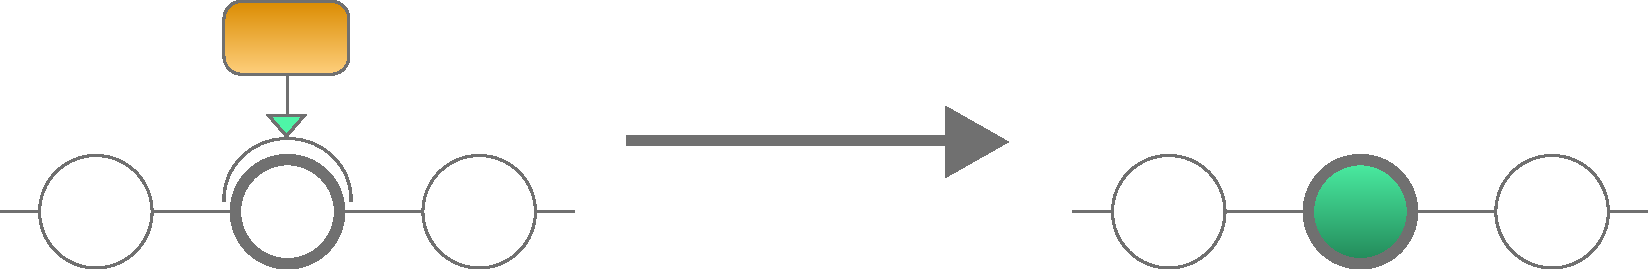
\includegraphics[width=\textwidth]{enzymes/random_a.pdf}
                        \end{minipage}
                        \vfill
                        \begin{minipage}{0.15\textwidth}
                            \caption*{\small \textbf{(b)}}
                        \end{minipage}
                        \begin{minipage}{0.8\textwidth}
                            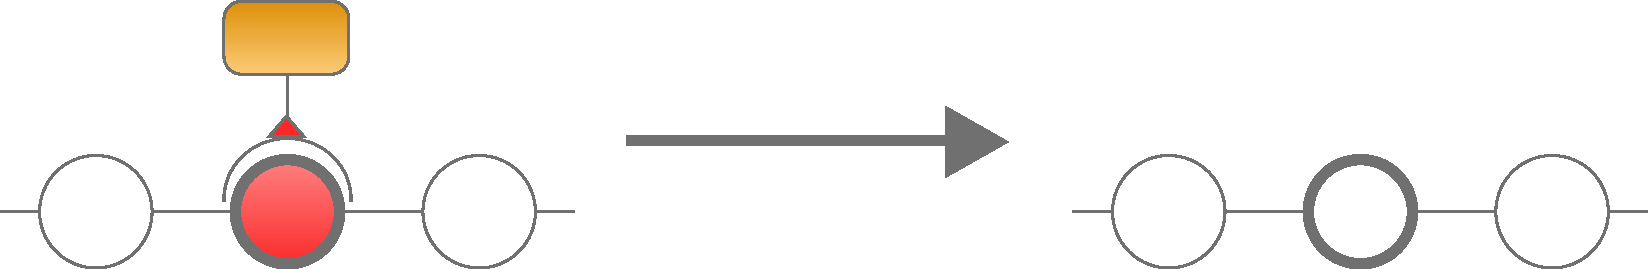
\includegraphics[width=\textwidth]{enzymes/random_b.pdf}
                        \end{minipage}
                    \end{minipage}
                    \caption{Simplified model of random modifier enzyme \textbf{(a)} acetylation addition \textbf{(b)} and methylation removal reactions. Acetylated nucleosomes are coloured in green, methylated nucleosomes are red and colourless ones are unmodified. Random modifier enzyme methylation addition and acetylation removal work analogically.}
                    \label{img:randomEnzymes}
                \end{figure}
                %

                %
                Random modifier enzymes' patterns do not have a context. However, a random methylation adder cannot bind to any already modified nucleosome, only to an unmodified one.
                %

                %
                Random modifier enzymes are not only “enzymes” in the true sense of the word when compared to the biological aspect of the model. They also exist in order to mimic the “noise” that is associated with such systems. Given that any nucleosome can be targeted by a specific random enzyme at any moment, these enzymes' association rate should be smaller than the other ones' in the system when trying to keep noise levels low.
                %
            %
            %
        %
        %
        \subsection{Enzyme rule sets}
            %
            This subsection provides an overview of the different enzyme rule sets used in the different simulations featured in this work. The rule sets are always kept constant throughout every section in the 'Results' chapter respectively, unless stated otherwise. The enzyme rule sets used are summarized in tab. \ref{tab:EnzymeRuleSets}.
            %

            %
            \begin{table}[htbp!]
                \centering
                \caption{Summary on whether an enzyme type was included and if the chromatin string was cyclic or not in the designated experiment presented in the indicated 'Results' section. \textbf{X} designates an affirmation.}
                \begin{tabular}{l|ccccc}
                                            & \ref{sec:ResNon-cooperative}  & \ref{sec:ResNonCyc} & \ref{sec:ResBistableSwitching}  & \ref{sec:ResBoundariesBistability}    \\\hline
                Random adders               & \textbf{X}                    & \textbf{X}          & \textbf{X}                      & \textbf{X}                            \\\hline
                Random removers             & \textbf{X}                    & \textbf{X}          & \textbf{X}                      & \textbf{X}                            \\\hline
                Linear adders               & \textbf{X}                    &                     &                                 &                                       \\\hline
                Linear removers             & \textbf{X}                    &                     &                                 &                                       \\\hline
                Cooperative adders          &                               & \textbf{X}          & \textbf{X}                      & \textbf{X}                            \\\hline
                Cooperative removers        &                               & \textbf{X}          &                                 &                                       \\\hline
                Cyclic                      &                               &                     & \textbf{X}                      & \textbf{X}                            \\\hline
                Non-cyclic                  & \textbf{X}                    & \textbf{X}          &                                 &                                       \\\hline
                \end{tabular}
                \label{tab:EnzymeRuleSets}
            \end{table}
           %
    %
    %
    \section{Simulation details}
    \label{sec:simulationDetails}
        %
        The input files for the performed \ed/ simulations can be found at \cite{Krecké2021}. In general, every \ed/ run needs three files: a \textit{statefile}, a \textit{rulefile} and a \textit{paramfile}. The \textit{statefile} contains the starting state of the nucleosome string. The \textit{rulefile} contains all specifications to the enzymes: their patterns, the modification pattern, the association rate and the dissociation rate. The \textit{paramfile} holds general information about the simulation itself with the most important one being the simulation time. This numeric parameter sets the exit condition for the algorithm.
        %

        %
        The simulation time changes significantly between some runs. This is due to Gillespie's algorithm's event-based time approach. Changing the enzyme set can result in a significantly different number of possible reactions during the simulation which can lead to very short simulation step numbers. Thus, in order to grant statistically significant runs, the simulation time was increased for certain runs, if the overall run time was empirically found to be too short.
        %

        %
        Furthermore, for reasons of performance and storage space, the graphs included in the results section were made from simulations with different simulation time. Preprocessing for the heatmaps was significantly more expensive than the other plots. Therefore, heatmaps were generated from \textit{short} runs, whereas the other plots were generated from \textit{long} runs. Meaning:
        %

        %
        \begin{itemize}
            \item \textit{short}: Every step (event) is plotted and metadata are used to plot association numbers and relative binding time (resulting in heatmaps).
            \item \textit{long}: Only every 1000th step is plotted. Given that the system is chaotic thanks to the random nature of the algorithm, regular plotting (e.g. every 1000th data point) results in a smoothing of the histogram because the chosen data points are more representative for the underlying distribution. Thus, there is no need for varying the skip length of 1000 throughout a run.
        \end{itemize}
        %
    %
    %
%
%